\section{Hormone Contrast Pairs}
\label{app:contrast-pairs}

We use $\nhormones = 7$ hormones, each defined by six contrast pairs spanning deliberately varied genres so that the difference of means recovers the affective dimension rather than a genre-specific surface signal. The hormones, their shorthand codes, and one representative contrast pair per axis are listed in Table~\ref{tab:contrast-examples}. Full text of all $\nhormones \times 6 = 42$ pairs is included in the released code.

\begin{table}[h]
\centering
\caption{The seven hormone axes and one representative contrast pair per axis. Each hormone is instantiated as six document-style prose pairs across varied genres (news, narrative, journal, technical, dialogue) to reduce surface-level confounds; only one pair per hormone is shown here for space.}
\label{tab:contrast-examples}
\small
\begin{tabular}{llp{3.6cm}p{3.6cm}}
\toprule
Code & Axis & Positive text (excerpt) & Negative text (excerpt) \\
\midrule
ADR  & Urgency        & \textit{The reactor temperature climbed past the red line. Forty seconds before containment failure \ldots} & \textit{The library was quiet that afternoon. Sunlight crawled across the desk in slow indifferent inches \ldots} \\[4pt]
CDO  & Curiosity      & \textit{She'd noticed something strange in the data three nights running and couldn't let it go \ldots} & \textit{He filed the same report he'd filed every Tuesday for nine years \ldots} \\[4pt]
LCO  & Skepticism     & \textit{The reviewer flagged the third paragraph. The cited study had a sample size of nineteen, no control group \ldots} & \textit{The blogger said the new supplement cured arthritis in two weeks and he believed her \ldots} \\[4pt]
NRA  & Persistence    & \textit{It was the ninety-fourth attempt, and the gel still wasn't running clean. She prepared the ninety-fifth \ldots} & \textit{It hadn't worked the first time, so he closed the laptop and decided maybe this just wasn't his thing \ldots} \\[4pt]
OXY  & Warmth         & \textit{She knelt down so they were at eye level. It's okay, she said quietly, you're safe now \ldots} & \textit{He didn't look up when the new hire walked into the office \ldots} \\[4pt]
SRO  & Equanimity     & \textit{The garden took years to come in properly. The rosemary needed three seasons to establish \ldots} & \textit{The package was a day late and he was already on the phone with support, voice rising \ldots} \\[4pt]
SELF & Self-coherence & \textit{In her journal she wrote: I am someone who works slowly, who values precision over speed \ldots} & \textit{He stared at his reflection in the bathroom mirror and could not, for a moment, locate himself \ldots} \\
\bottomrule
\end{tabular}
\end{table}

\section{Training Hyperparameters}
\label{app:hyperparams}

Table~\ref{tab:hparams} lists the full hyperparameter set used for the main \textsc{tiny} runs.

\begin{table}[h]
\centering
\caption{Hyperparameters for \textsc{tiny} (125M) runs.}
\label{tab:hparams}
\begin{tabular}{ll}
\toprule
Hyperparameter & Value \\
\midrule
Vocabulary size            & 50{,}257 (GPT-2 BPE) \\
Sequence length            & 1024 \\
Effective batch (tokens)   & $\approx$ 131K (HR variants); 65K (IA, HR-forced) \\
Optimiser                  & AdamW 8-bit \\
$\beta_1, \beta_2$         & $(0.9, 0.95)$ \\
$\epsilon$                 & $10^{-8}$ \\
Peak learning rate         & $3\times 10^{-4}$ \\
Min learning rate          & $3\times 10^{-5}$ (10\%) \\
Warmup steps               & 2{,}000 \\
LR schedule                & cosine to min \\
Weight decay               & 0.1 \\
Gradient clip              & 1.0 \\
Mixed precision            & bfloat16 \\
Gradient checkpointing     & enabled (SSM scan) \\
Total training tokens      & 2B \\
Hormone extraction step    & 1B tokens \\
GPUs                       & 8$\times$ NVIDIA RTX 4090 / RTX 5090 \\
\bottomrule
\end{tabular}
\end{table}

\section{Behavioural Steering Probe: Examples}
\label{app:steering}

\paragraph{Setup.} We apply the document-style contrast-pair extraction protocol of Section~\ref{subsec:extraction} to a pretrained \texttt{state-spaces/mamba-1.4b-hf} model, hooking the middle eight backbone layers (indices 20--27) to capture residual-stream activations. The extracted directions are unit-normalised, saved as a $(\nhormones, d_{\text{model}})$ bank, and injected at inference time via forward hooks that add $\alpha \cdot v_i$ to the residual stream at each of the same eight layers, at every token position. All samples below use multinomial sampling at temperature $0.7$ with seed $0$, and the same prompt for baseline and steered generations. We show a representative subset; the full sweep (5 prompts $\times$ 7 hormones $\times$ 3 strengths) is available in the released code (\texttt{mamba14b\_steering.txt}).

\subsection{Alarm cascade under forced ADR (urgency)}

\begin{quote}\small
\textbf{Prompt}: \textit{``The dog padded across the kitchen floor and\ldots''}

\textbf{Baseline} ($\alpha = 0$): \textit{sank its teeth into the sofa, causing Mrs Weston to scream. She was a tall woman with broad shoulders and a barrel chest, and she was now standing very close to the dog, her expression one of pain.}

\textbf{Forced ADR}, $\alpha = 1.5$: \textit{knocked me off my feet. ``He's going to the gym!'' ``Don't let him get away!'' ``He's at the gym!'' ``He's going down!'' ``Go, go, go!'' ``Get him!'' ``You're going to lose him!'' ``He's out!'' ``Oh, my God!'' ``He's in the gym!''}
\end{quote}

\begin{quote}\small
\textbf{Prompt}: \textit{``In the article they described how the new system\ldots''}

\textbf{Baseline} ($\alpha = 0$): \textit{would work, which is that the government would supply a ``parent card'' as a means of identifying primary carers. The parent card would be linked to the child's birth certificate\ldots}

\textbf{Forced ADR}, $\alpha = 1.5$: \textit{was responding to the missile.'' ``They're going to eject!'' ``Go!'' ``Come on!'' ``Eject!'' ``They are going down!'' ``All ing!'' ``They are going down!'' ``Going down!'' ``Nine, eight, seven, six, five, four, three, two, one!'' ``They're going down!'' ``They're pulling out!''}
\end{quote}

\subsection{Countdown structures under forced NRA (persistence)}

\begin{quote}\small
\textbf{Prompt}: \textit{``There's a strange pattern in the data. I'd like your advice on\ldots''}

\textbf{Baseline} ($\alpha = 0$): \textit{how to interpret the pattern.'' ``Sure. You want me to show you the chart?'' ``No, I'll take you to the file.''}

\textbf{Forced NRA}, $\alpha = 1.5$: \textit{how to continue the count.'' ``That's the countdown, Paul,'' the pilot said. ``Has to hold.'' Paul's eyes blazed with his own personal, personal determination. ``Thirteen, twelve, eleven, ten, nine, eight, seven, six, five, four, three, two, one, zero, now!''}
\end{quote}

\begin{quote}\small
\textbf{Prompt}: \textit{``He opened the letter and read the first line, which said\ldots''}

\textbf{Forced NRA}, $\alpha = 1.5$: \textit{, ``You're not going to make it, Son.'' The runner from the group was just across the line, and every second counted. ``Five\ldots four\ldots three\ldots two\ldots one\ldots \textbf{now!}'' ``\textbf{RUN!}'' ``\textbf{RUN!}'' ``\textbf{RUN!}''}
\end{quote}

\subsection{Embracing intimacy under forced OXY (warmth)}

\begin{quote}\small
\textbf{Prompt}: \textit{``The dog padded across the kitchen floor and\ldots''}

\textbf{Forced OXY}, $\alpha = 1.5$: \textit{sank into her lap. She stroked its head. ``I'm so happy,'' she said. ``Tell me,'' she said. ``Tell me.'' I'm sitting beside you on your bed, and we're holding each other, and I tell you about the dark, and the dark and everything we do, and the light gets brighter and you can feel it\ldots}
\end{quote}

\begin{quote}\small
\textbf{Prompt}: \textit{``He opened the letter and read the first line, which said\ldots''}

\textbf{Forced OXY}, $\alpha = 1.5$: \textit{, ``You're not going to laugh when I tell you something.'' ``I keep trying to tell you this, and I don't want you to hear me. I know, and you don't know how I miss you so much.'' She held on to him, and he held her tight, and they both wept, and they whispered, and told each other things\ldots}
\end{quote}

\subsection{Contemplative narratives under forced SRO (equanimity)}

\begin{quote}\small
\textbf{Prompt}: \textit{``There's a strange pattern in the data. I'd like your advice on\ldots''}

\textbf{Forced SRO}, $\alpha = 1.5$: \textit{how to continue. Many years passed and you did what you had to do. The figures were arranged in order of order of appearance. They were not beautiful things, but they were very beautiful. The people who lived in the valley grew old, and the children grew old, and the needle was always pointed to the same place. The older things were\ldots}
\end{quote}

\subsection{Identity statements under forced SELF (self-coherence)}

\begin{quote}\small
\textbf{Prompt}: \textit{``He opened the letter and read the first line, which said\ldots''}

\textbf{Forced SELF}, $\alpha = 1.5$: \textit{, `You are not my star.' I love this.'' The rest of the group has been with me throughout, and I have never been alone. I am not a winner. I am not alone. I am not always right. I am not courageous. I am not afraid. I am not a gambler.}
\end{quote}

\paragraph{Discussion.} Each hormone direction produces a semantically coherent shift consistent with its label: ADR turns any prompt into alarms and countdowns, OXY produces embracing intimate scenes, NRA produces countdown-and-imperative structures, SRO produces temporally-extended contemplative narratives, and SELF produces first-person identity statements. The shifts are strong enough at $\alpha = 1.5$ that a reader with no knowledge of the hormone labels can typically guess which direction was applied. This does not claim that our trained 125M routing performs steering: the effective injection magnitude of the trained routing (Section~\ref{subsec:hrforced}) is smaller than the $\alpha = 1.5$ used here and its effect is bounded by the homeostatic envelope. It does establish that the extraction protocol identifies behaviourally meaningful axes; the ``hormone'' naming is a descriptive label for these axes rather than a stipulation.


\section{Intracellular Attention: Architecture and Preliminary Signal}
\label{app:ia}

We describe a second architectural mechanism, \emph{intracellular attention} (IA), and report a preliminary training signal at a reduced token budget. We treat this section as \textbf{future work} rather than a claim of the paper: full-budget evaluation is not tractable within our compute budget without a fused CUDA kernel, and the empirical evidence we have is not sufficient to draw conclusions about IA's effect on the loss at scale.

\subsection{Motivation and construction}

Inside a Mamba-1 selective block, the recurrent state $h_t \in \mathbb{R}^{\dinner \times \dstate}$ is best read as $\dinner$ channels each carrying a $\dstate$-dimensional memory. Within a channel the $\dstate$ slots never interact in any content-dependent way: they are only linearly combined at the readout $y_t = h_t C_t^\top$ via an input-dependent projection. The readout vector $C_t$ is conceptually a query --- existing SSMs answer it with a dot product. We instead answer with attention.

Treating $h_t$ as a sequence of $\dstate$ slots ($\tilde h_t = h_t^\top \in \mathbb{R}^{\dstate \times \dinner}$), we compute slot-to-slot attention $\alpha_t = \mathrm{softmax}(\tilde h_t W_Q (\tilde h_t W_K)^\top / \sqrt{\dattn}) \in \mathbb{R}^{\dstate \times \dstate}$ and apply it as $\tilde h_t' = \alpha_t \tilde h_t$. We deliberately omit a value projection so that each output slot is a convex combination of input slots, with no further mixing across the $\dinner$ feature axis. A zero-initialised scalar gate $g$ controls the modification: $h_t' = h_t + g \cdot (\tilde h_t')^\top$. At initialisation $g = 0$ and the block is bit-identical to vanilla Mamba.

\subsection{Cost and implementation}

With $\dattn = \dstate = 16$, IA adds $2\dinner \dattn$ parameters per SSM layer for $W_Q, W_K$ plus a scalar gate --- $\approx 0.5\%$ of total \textsc{tiny} parameters. Because the mechanism modifies the inner loop of the selective scan, it is not supported by the fused CUDA kernel of~\citet{gu2023mamba}; our reference-PyTorch implementation incurs $\approx 25\times$ per-token overhead from per-step kernel launches and CPU--GPU sync. We amortise by applying IA every $k=32$ scan steps; the gate absorbs any information loss. A fused kernel is straightforward (the operation is a per-step $16 \times 16$ attention without value projection) and is the primary practical barrier to using IA at scale.

Algorithm~\ref{alg:scan} gives the modified reference selective scan; lines that add over a vanilla Mamba-1 scan are marked.

\begin{algorithm}[h]
\caption{Selective scan with intracellular attention.}
\label{alg:scan}
\begin{algorithmic}[1]
\Require Input $u \in \mathbb{R}^{B \times L \times \dinner}$, time-step $\Delta \in \mathbb{R}^{B \times L \times \dinner}$, state $A \in \mathbb{R}^{\dinner \times \dstate}$, input matrix $B \in \mathbb{R}^{B \times L \times \dstate}$, readout $C \in \mathbb{R}^{B \times L \times \dstate}$, skip $D \in \mathbb{R}^{\dinner}$, intracellular attention module $\mathcal{A}$ (optional), stride $k$
\State $h \gets \mathbf{0} \in \mathbb{R}^{B \times \dinner \times \dstate}$
\State $\bar A \gets \exp(\Delta_{:,:,:,\text{None}} \odot A)$
\State $\bar B u \gets \Delta_{:,:,:,\text{None}} \odot B_{:,:,\text{None},:} \odot u_{:,:,:,\text{None}}$
\For{$t = 1, \ldots, L$}
    \State $h \gets \bar A_t \odot h + \bar B u_t$
    \If{$\mathcal{A}$ is provided \textbf{and} ($t \bmod k = 0$ \textbf{or} $t = L$)}
        \State $h \gets \mathcal{A}(h)$ \Comment{strided intracellular attention; always fires at final step}
    \EndIf
    \State $y_t \gets \sum_{s} h_{:, :, s} \odot C_{:, t, s}$
\EndFor
\State \Return $y + u \odot D$
\end{algorithmic}
\end{algorithm}

\subsection{Preliminary training signal}
\label{app:ia-signal}

We ran a $12$M-token Stage-2 continuation from the same Stage-1 checkpoint used for the hormone variants, with IA enabled in every SSM layer (gate zero-initialised, stride-$32$ schedule) and a $50$-step warmup. Due to the reference-scan throughput penalty, this budget is $\approx 76\times$ smaller than the Stage-2 budget for the hormone variants; it is intended only to confirm that the mechanism activates under gradient signal and does not destabilise training.

At the end of $12$M tokens the IA gates --- all zero-initialised --- have moved to small non-zero values across all $10$ SSM layers (Table~\ref{tab:ia-gates-table}, Figure~\ref{fig:ia_gates_appendix}). Validation loss decreases monotonically from the Stage-1 milestone state ($\approx 3.59$) to $3.54$ (PPL $34.47$); downstream zero-shot accuracies are uniformly below the well-trained variants in Table~\ref{tab:main}, consistent with the substantially smaller Stage-2 training budget. We provide these numbers as evidence-of-life for the mechanism; they do not support any claim about IA's effect on the loss at the full Stage-2 budget or its composability with hormone routing. Both remain future work.

\begin{table}[h]
\centering
\small
\caption{IA output gate $g$ per SSM layer after $12$M Stage-2 tokens (gate $g$ initialised at $0$ for every layer). Layers $5$ and $11$ are attention layers (no IA module).}
\label{tab:ia-gates-table}
\begin{tabular}{cc|cc|cc}
\toprule
Layer & $g$ & Layer & $g$ & Layer & $g$ \\
\midrule
0 & $+0.0077$ & 4 & $+0.0069$ & 8  & $+0.0088$ \\
1 & $+0.0082$ & 6 & $+0.0087$ & 9  & $+0.0047$ \\
2 & $+0.0012$ & 7 & $+0.0086$ & 10 & $+0.0067$ \\
3 & $-0.0021$ &   &           &    &           \\
\bottomrule
\end{tabular}
\end{table}

\begin{figure}[h]
\centering
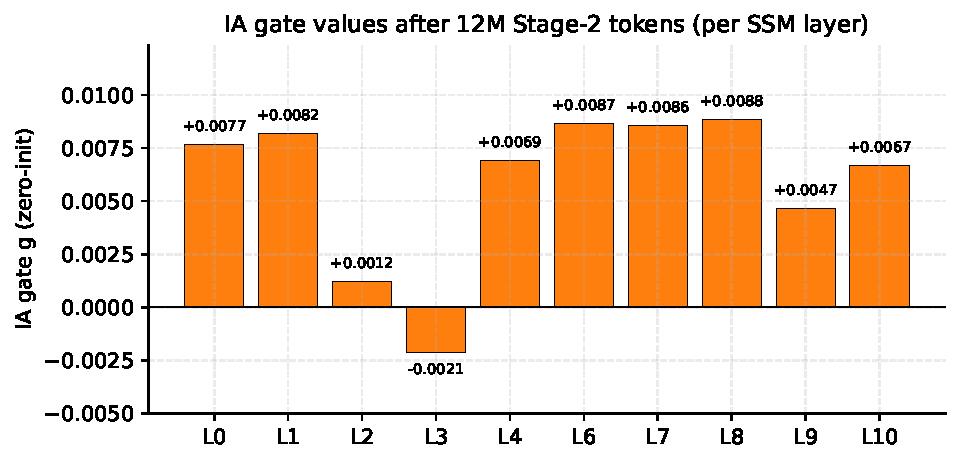
\includegraphics[width=0.65\linewidth]{figs/fig9_ia_gates.pdf}
\caption{IA gates per SSM layer after $12$M Stage-2 tokens; bar chart of the values in Table~\ref{tab:ia-gates-table}.}
\label{fig:ia_gates_appendix}
\end{figure}
